\documentclass[aps,prd,amsmath,superscriptaddress,floatfix,nofootinbib]{revtex4-2}

% math packages
\usepackage{mathrsfs}
\usepackage{amsfonts}
\usepackage{amsmath}
\usepackage{amssymb}
\usepackage{bm}
\usepackage{slashed}
\usepackage{physics}

\newcommand{\diff}[1]{{\rm d} #1}

% float packages
\usepackage{graphicx}
\graphicspath{{./figures}}
\usepackage[caption=false]{subfig}

% miscellaneous
\usepackage{siunitx}
\usepackage{xcolor}
\usepackage[colorlinks=true,citecolor=green,linkcolor=blue,urlcolor=blue]{hyperref}

% ref macros
\newcommand{\eref}[1]{Eq.~(\ref{eq:#1})}
\newcommand{\erefs}[2]{Eqs.~(\ref{eq:#1})--(\ref{eq:#2})}
\newcommand{\fref}[1]{Fig.~\ref{fig:#1}}
\newcommand{\frefs}[2]{Figs.~\ref{fig:#1}--\ref{fig:#2}}
\newcommand{\sref}[1]{Sec.~\ref{sec:#1}}
\newcommand{\ssref}[1]{Sec.~\ref{ss:#1}}
\newcommand{\sssref}[1]{Sec.~\ref{sss:#1}}
\newcommand{\tref}[1]{Table~\ref{tab:#1}}

\begin{document}

\title{Notes on PVDIS}
\author{Richard Whitehill}
\date{\today}
\maketitle

\section{Overview of Deep-Inelastic Scattering (DIS)}
\label{sec:overview-of-deep-inelastic-scattering}

The deep-inelastic scattering process refers generally to the lepton-nucleon collision $\ell N \rightarrow \ell' X$, where $X$ is the unobserved hadronic final state particle(s).
Since the original experiments at SLAC, DIS has been one of the most fruitful methods by which we have learned about the structures of the proton and neutron, and it will continue to be so for the foreseeable future, especially given the iminent operation of the Electron-Ion Collider (EIC) at Brookhaven national lab, which will give unprecedented access to a larger kinematic phase space.

For these notes, we restrict our attention to neutral-current processes, and in particular, we only consider contributions from processes that enter at first-order in boson exchanges between the lepton and nucleon (as shown in \fref{DIS-one-photon}).
In doing so, we have the following kinematic definitions:
\begin{itemize}
    \item $\displaystyle \nu = \frac{P \cdot q}{M} = E - E'$ is the energy lost by the lepton in the nucleon rest frame.
    \item $Q^2 - -q^2 = -(\ell - \ell')^2$ is the virtuality of the virtual photon.
    \item $\displaystyle x = \frac{Q^2}{2 P \cdot q} = \frac{Q^2}{2 M \nu}$ is the typical Bjorken scaling variable.
    \item $\displaystyle y = \frac{P \cdot q}{P \cdot \ell} = \frac{\nu}{E}$ is the inelasticity variable.
    \item $\displaystyle W^2 = (P + q)^2 = M^2 + Q^2 \Big( 1 - \frac{1}{x} \Big)$ is the invariant mass of the hadronic final state.
    \item $\displaystyle s = (P + \ell)^2 = M^2 + \frac{Q^2}{xy}$ is the squared center of mass energy of the lepton-nucleon system.
\end{itemize}
Note that DIS is characterized by the following kinematic constraints: $Q^2, W^2 \gg M^2$.

\begin{figure}[h!b]
\begin{center}
    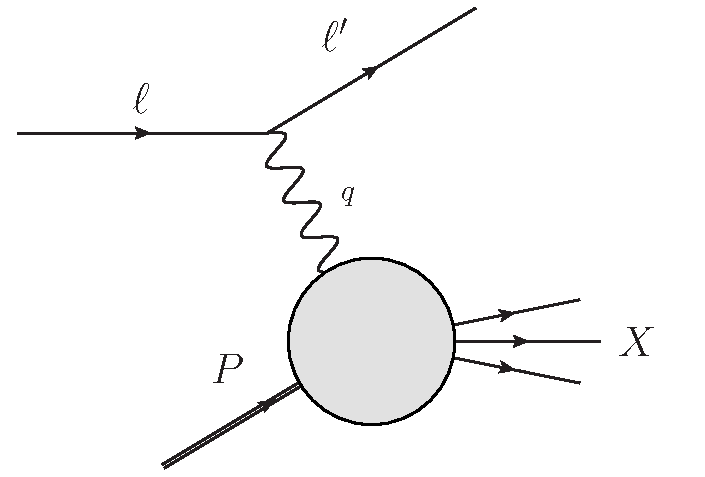
\includegraphics[width=0.5\paperwidth]{./figures/DIS_generic.pdf}
    \caption{Generic feynman diagram representing the DIS process in the one-``photon'' exchange approximation.}
    \label{fig:DIS-one-photon}
\end{center}
\end{figure}

Using Fermi's Golden rule, we can write the cross section for this process (summing and integrating over the hadronic final states) as
\begin{eqnarray}
    \label{eq:xsec-general}
    \diff \sigma = \frac{1}{4 P \cdot \ell} \frac{\diff^3 {\bm \ell'}}{(2\pi)^{3} 2E'} \sum_{X} \int \Big( \prod_{i \in X} \frac{\diff^3 {\bm P_{i}}}{(2\pi)^3 2E_{i}} \Big) (2\pi)^{4} \delta^{(4)}(P + q - P_{X}) |{\cal M}|^2 
,\end{eqnarray}
Rewriting, we find
\begin{eqnarray}
    \label{eq:xsec-rewritten}
    \frac{\diff \sigma}{\diff E' \, \diff \Omega} = \frac{1}{2(s-M^2)} \frac{E'}{2(2\pi)^3} \sum_{X} \int \diff \Phi_{X} (2\pi)^{4} \delta^{(4)}(P+q-P_{X}) |{\cal M}|^2
.\end{eqnarray}

At this juncture, we analyze the form of the scattering amplitude.
The full amplitude is given as a sum of contributions from the processes mediated by a virtual photon and $Z$-boson, respectively,
\begin{eqnarray}
    \label{eq:DIS-amp}
    {\cal M} = {\cal M}_{\gamma} + {\cal M}_{Z}
,\end{eqnarray}
where $\displaystyle {\cal M}_{\gamma(Z)} = \bra{\ell',s'} j_{\mu}^{\gamma(Z)} \ket{\ell,s} \frac{g^{\mu\nu}}{Q^2} \bra{X} J_{\nu}^{\gamma(Z)} \ket{P,S} = \frac{1}{Q^2} \bra{\ell',s'} j_{\mu}^{\gamma(Z)} \ket{\ell,s} \bra{X} J^{\mu}_{\gamma(Z)} \ket{P,S}$, where $j_{\mu}^{\gamma(Z)}$ and $J_{\mu}^{\gamma(Z)}$ are electromagnetic (weak) lepton and nucleon currents.
Note that the factor $g^{\mu\nu}/Q^2$ is the virtual boson propagator, which is exact when the boson is a photon and approximate when the virtual particle is a $Z$-boson ($Q^2 \ll M_{Z}^2$).
The squared amplitude is then
\begin{eqnarray}
    \label{eq:DIS-sq-amp}
    |{\cal M}|^2 = |{\cal M}_{\gamma}|^2 + {\cal M}_{\gamma}^{*}{\cal M}_{Z} + {\cal M}_{Z}^{*}{\cal M}_{\gamma} + |{\cal M}_{Z}|^2
.\end{eqnarray}
Using the current matrix elements above, we can separate the leptonic and hadronic contributions to the cross section as a tensor product:
\begin{eqnarray}
    \label{eq:xsec-lep-had-tensors}
    \frac{\diff \sigma}{\diff E' \, \diff \Omega} = \frac{1}{2(s-M^2)} \frac{E'}{2(2\pi)^3} \frac{e^4}{Q^{4}} \sum_{i} [\eta_{i} L_{\mu\nu}^{i} (4\pi W^{\mu\nu}_{i})]
,\end{eqnarray}
where $i \in \{ \gamma, \gamma Z, Z \}$, $L_{\mu\nu}^{i}$ is the leptonic tensor, $W^{\mu\nu}_{i}$ is the hadronic tensor (where the factor of $4\pi$ is a normalization factor introduced by convention), and $\eta_{i}$ collects kinematic factors from the squared matrix elements.
We write down the kinematic factors $\eta_{i}$ with the corresponding lepton tensor $L_{\mu\nu}^{i}$:
\begin{itemize}
    \item $\eta_{\gamma} = 1$ and $L_{\mu\nu} = 2(\ell^{\mu} \ell'_{\nu} + \ell'_{\mu} \ell_{\nu} - g_{\mu\nu} \ell \cdot \ell' - i \lambda_{\ell} \epsilon_{\mu\nu\alpha\beta} \ell^{\alpha}\ell'^{\beta})$
    \item $\displaystyle \eta_{\gamma Z} = \Big( \frac{G_{F}M_{Z}^2}{2\sqrt{2} \pi \alpha} \Big) \Big( \frac{Q^2}{Q^2 + M_{Z}^2} \Big)$ and $L_{\mu\nu}^{\gamma Z} = (g_{V}^{\ell} - \lambda g_{A}^{\ell})L_{\mu\nu}^{\gamma}$
    \item $\eta_{Z} = \eta_{\gamma Z}^2$ and $L_{\mu\nu}^{Z} = (g_{V}^{\ell} - \lambda g_{A}^{\ell})^2 L_{\mu\nu}^{\gamma}$
\end{itemize}
Note that $g_{V}^{\ell} = {\color{red} \bm ?}$ and $g_{A}^{\ell} = {\color{red} \bm ?}$ are the vector and axial weak couplings for lepton $\ell$, respectively, and $\lambda_{\ell}$ is the helicity of the lepton (assuming longitudinal polarization).
Finally, we write down the definition of the hadronic tensor as
\begin{subequations}
    \label{eq:hadron-tensor-def}
    \begin{eqnarray}
        W^{\mu\nu}_{\gamma} = \frac{1}{4\pi} \sum_{X} \int \diff \Phi_{X} \delta_{\rm PS}^{(4)} \bra{P,S} J^{\mu \, \dagger}_{\gamma} \ket{X} \bra{X} J^{\nu}_{\gamma} \ket{P,S}
    \end{eqnarray}
    \begin{align}
        W^{\mu\nu}_{\gamma Z} = \frac{1}{4\pi} \sum_{X} \int \diff \Phi_{X} \delta_{\rm PS}^{(4)} \big[ &\bra{P,S} J^{\mu \, \dagger}_{\gamma} \ket{X} \bra{X} J^{\nu}_{Z} \ket{P,S} \notag \\
                                                                                                        &+ \bra{P,S} J^{\mu \, \dagger}_{Z} \ket{X} \bra{X} J^{\nu}_{\gamma} \ket{P,S} ]
    \end{align}
    \begin{eqnarray}
        W^{\mu\nu}_{Z} = \frac{1}{4\pi} \sum_{X} \int \diff \Phi_{X} \delta_{\rm PS}^{(4)} \bra{P,S} J^{\mu \, \dagger}_{Z} \ket{X} \bra{X} J^{\nu}_{Z} \ket{P,S}
    ,\end{eqnarray}
\end{subequations}
where $\delta^{(4)}_{\rm PS} = (2\pi)^{4} \delta^{(4)}(P+q-P_{X})$.
Generally, we can parameterize the hadronic tensor in terms of structure functions, ensuring that it obeys current conservation (i.e. $\partial_{\mu}J^{\mu} = 0 \Leftrightarrow q_{\mu}W^{\mu\nu} = 0$) and Lorentz covariance, as
\begin{eqnarray}
\label{eq:hadronic-tensor-structure-functions}
\begin{aligned}
    W^{\mu\nu} &= -\tilde{g}^{\mu\nu} F_{1}(x,Q^2) + \tilde{P}^{\mu}\tilde{P}^{\nu} \frac{F_{2}(x,Q^2)}{P \cdot q} - i \epsilon^{\mu\nu\alpha\beta} \frac{q^{\alpha}P^{\beta}}{2 P \cdot q} F_{3}(x,Q^2) \\
               &+ i\epsilon^{\mu\nu\alpha\beta} \frac{q^{\alpha}}{P \cdot q} \Big[ S^{\beta} g_{1}(x,Q^2) + \Big( S^{\beta} - \frac{S \cdot q}{P \cdot q} \Big) g_{2}(x,Q^2) \Big] \\
               &+ \frac{1}{P \cdot q} \Big[ \frac{1}{2} \Big( \tilde{P}^{\mu}\tilde{S}^{\nu} + \tilde{S}^{\mu}\tilde{P}^{\nu} \Big) - \frac{S \cdot q}{P \cdot q} \tilde{P}^{\mu}\tilde{P}^{\nu} \Big] g_{3}(x,Q^2) \\
               &+ \frac{S \cdot q}{P \cdot q} \Big[ \tilde{P}^{\mu}\tilde{P}^{\nu} \frac{g_{4}(x,Q^2)}{P \cdot q} - \tilde{g}^{\mu\nu} g_{5}(x,Q^2) \Big]
,\end{aligned}
\end{eqnarray}
where $\displaystyle \tilde{g}^{\mu\nu} = g^{\mu\nu} - \frac{q^{\mu}q^{\nu}}{q^2}$ and $\tilde{P}^{\mu} = \tilde{g}^{\mu\nu} P_{\nu}$.
Furthermore, we note that $S$ is the nucleon 4-vector with $S^2 = -M^2$ and $S \cdot P = 0$, and lastly, we note that $F_{j}(x,Q^2)$ and $g_{j}(x,Q^2)$ are the unpolarized and polarized\footnote{It should be noted that $W^{\mu\nu} = W^{\mu\nu}(P,q,S)$, and unpolarized structure functions appear in the sum $W^{\mu\nu}(P,q,S) + W^{\mu\nu}(P,q,-S)$ while polarized structure functions appear in the difference $W^{\mu\nu}(P,q,S) - W^{\mu\nu}(P,q,-S)$.} dimensionless Bjorken-scaling structure functions, respectively.

Now, we can change variables from $(E',\Omega)$ to $(x,y)$, which gives us the conventional DIS cross section as
\begin{eqnarray}
\label{eq:xsec-xy}
    \frac{\diff \sigma}{\diff x \, \diff y} = \frac{Q^2}{x} \frac{\pi}{E'} \frac{\diff \sigma}{\diff E' \, \diff \Omega} = \frac{2 \pi \alpha^2 y}{Q^4} \sum_{i} \eta_{i} L_{\mu\nu}^{i}W_{i}^{\mu\nu}
,\end{eqnarray}
where we have used the relation $e^2 = 4\pi\alpha$.
Note that $\diff \sigma = \diff \sigma(\lambda_{\ell}, S)$ depends on the helicity of the electron (in the initial state) and spin of the nucleon.
We can therefore define cross sections that depend on exclusively on the spin of either the electron or the nucleon.
When we refer to the polarization of a cross section, we explicitly refer to the polarization of the nucleon.
Therefore, the unpolarized cross section is given by
\begin{eqnarray}
\label{eq:upol-xsec}
\begin{aligned}    
    \frac{\diff \sigma_{U}}{\diff x \, \diff y} &= \frac{1}{2} \Bigg[ \frac{\diff \sigma(\lambda_{\ell},S)}{\diff x \, \diff y} + \frac{\diff \sigma(\lambda_{\ell},S)}{\diff x \, \diff y} \Bigg] = \frac{2 \pi \alpha^2 y}{Q^{4}} \sum_{i} \eta_{i} L_{\mu\nu}^{i} W^{\mu\nu}_{U,i} \\
                                                &= \frac{4 \pi \alpha^2}{x y Q^2} \Bigg[ xy^2 F_{1}^{\rm NC}(x,Q^2) \Bigg( 1 - y - \frac{x^2 y^2 M^2}{Q^2} \Bigg) F_{2}^{\rm NC}(x,Q^2) {\color{red} - \lambda_{\ell} x \Bigg( y - \frac{y^2}{2} \Bigg)} F_{3}^{\rm NC}(x,Q^2) \Bigg]
.\end{aligned}
\end{eqnarray}
where $W^{\mu\nu}_{U} = \frac{1}{2} [ W^{\mu\nu}(P,q,S) + W^{\mu\nu}(P,q,-S) ]$ and 
\begin{subequations}    
\label{eq:NC-upol-structure-funcs}
\begin{eqnarray}
    \label{F1-NC}
    F_{1}^{\rm NC} = 
,\end{eqnarray}
\begin{eqnarray}
    \label{eq:F2-NC}
    F_{2}^{\rm NC} = 
,\end{eqnarray}
\begin{eqnarray}
    \label{eq:F3-NC}
    F_{3}^{\rm NC}
.\end{eqnarray}
\end{subequations}
Finally, the polarized cross section is given by ({\color{red} This equation needs to be updated once it is derived/verified})
\begin{eqnarray}
    \label{eq:pol-xsec}
    \frac{\diff \sigma_{U}}{\diff x \, \diff y} = \frac{1}{2} \Bigg[ \frac{\diff \sigma(\lambda_{\ell},S)}{\diff x \, \diff y} - \frac{\diff \sigma(\lambda_{\ell},S)}{\diff x \, \diff y} \Bigg] = \frac{2 \pi \alpha^2 y}{Q^{4}} \sum_{i} \eta_{i} L_{\mu\nu}^{i} W^{\mu\nu}_{P,i}
,\end{eqnarray}
where $W^{\mu\nu}_{P} = \frac{1}{2} [ W^{\mu\nu}(P,q,S) - W^{\mu\nu}(P,q,-S) ]$.
Finally, before moving on, we define
\begin{eqnarray}
    \label{eq:ratio}
    R^{i} = \frac{\sigma_{L}}{\sigma_{T}} = \frac{F_{2}^{i}}{2xF_{1}^{i}} r^2 - 1
,\end{eqnarray}
where $r^2 = 1 + Q^2/\nu^2$ and $\sigma_{L}$ and $\sigma_{T}$ are the longitudinal and transverse photoabsorption cross sections.


\section{The Parton Model}
\label{sec:the-naive-parton-model}

In the previous section, we outlined the calculation of the hadronic tensor and differential cross sections at the structure function level.
In this section, we outline the calculation of these quantities at the parton level, using a factorization framework.
At large $Q^2$, we can write the hadronic tensor as a convolution of hard scattering amplitudes and parton distribution functions (PDFs)\footnote{Neglecting higher order $m_{q}/Q$ corrections}:
\begin{subequations}
\label{eq:factorizations}
\begin{eqnarray}
    \label{eq:upol-had-tens-factorization}
    W^{\mu\nu}_{U} = \sum_{i} \int_{0}^{1} \frac{\diff \xi}{\xi} \widehat{W}^{\mu\nu}_{U}(\hat{x},Q^2) f_{i/P}(\xi,\mu^2)
\end{eqnarray}
and
\begin{eqnarray}
    \label{eq:pol-had-tens-factorization}
    W^{\mu\nu}_{P} = \sum_{i} \int_{0}^{1} \frac{\diff \xi}{\xi} \widehat{W}^{\mu\nu}_{P}(\hat{x},Q^2) \Delta f_{i/P}(\xi,\mu^2)
,\end{eqnarray}
\end{subequations}
where $\widehat{W}^{\mu\nu}$ is the partonic tensor (defined as the partonic analogue to the leptonic tensor), $(\Delta)f_{i/N}$ is the (polarized) unpolarized PDF for a parton of type $i$ in nucleon $N$, $\xi$ is the parton momentum fraction defined by $p = \xi P$, $\hat{x} = x/\xi$ is the partonic analogue to Bjorken-$x$, and $\mu$ is the renormalization scale for the PDFs (usually set such that $\mu^2 = Q^2$).
In the following text, we are interested in computing the hadronic structure functions in this factorization framework.
It is noted that several components go into the computation of the factorization integrand and the extraction of the structure functions.
Since these notes are focused on the phenomenology of PVDIS, we make no attempt to discuss the determination of the PDFs.
We simply utilize those PDFs, which were obtained from previous global QCD analyses, assuming that these studies were competent.
In the next sections, we outline the calculation of the partonic tensor (\ssref{calculation-of-the-partonic-tensor}) and the determination of the hadronic structure functions (\ssref{determination-of-the-hadronic-structure-functions}).

\subsection{Calculation of the partonic tensor}
\label{ss:calculation-of-the-partonic-tensor}

The partonic structure tensor is calculated as the squared amplitude for the virtual compton scattering process, shown in \fref{virtual-compton-scattering}, as
\begin{eqnarray}
    \label{eq:partonic-tensor}
    \widehat{W}^{\mu\nu}_{i} = \sum_{\rm graphs} {\cal M}^{\mu \, \dagger}_{i} {\cal M}^{\nu}_{i}
.\end{eqnarray}
In this work, we compute the partonic tensor at leading order, where the leading order process is simply $\gamma^{*} (q) + q (p) \rightarrow q (p')$ (shown in \fref{virtual-compton-scattering-LO}), which gives
\begin{subequations}    
\label{eq:partonic-tensor-LO}
\begin{eqnarray}
    \widehat{W}^{\mu\nu}_{\gamma} = \int \diff \Pi \, \Bigg\{ \sum_{s'} [ \bar{u}(p',s') \gamma^{\mu} u(p,s) ]^{*}[ \bar{u}(p',s') \gamma^{\nu} u(p,s) ] \Bigg\}
\end{eqnarray}
\begin{eqnarray}
\begin{aligned}
    \widehat{W}^{\mu\nu}_{\gamma Z} = \int \diff \Pi \, \Bigg\{ \sum_{s'} ( [ &\bar{u}(p',s') ( g_{V}^{i} - g_{A}^{i} \gamma^{5} ) \gamma^{\mu} u(p,s) ]^{*}[ \bar{u}(p',s') \gamma^{\nu} u(p,s) ]  \\
                                                                            &+ [ \bar{u}(p',s') \gamma^{\mu} u(p,s) ]^{*}[ \bar{u}(p',s') \gamma^{\nu} ( g_{V}^{i} - g_{A}^{i} \gamma^{5} ) u(p,s) ] ) \Bigg\}
\end{aligned}
\end{eqnarray}
\begin{eqnarray}
    \widehat{W}^{\mu\nu}_{Z} = \int \diff \Pi \, \Bigg\{ \sum_{s'} [ \bar{u}(p',s') \gamma^{\mu} ( g_{V}^{i} - g_{A}^{i} \gamma^{5} ) u(p,s) ]^{*}[ \bar{u}(p',s') \gamma^{\nu} ( g_{V}^{i} - g_{A}^{i} \gamma^{5} ) u(p,s) ] \Bigg\}
\end{eqnarray}

\end{subequations}
For the above tensors, note that
\begin{eqnarray}
    \label{eq:momentum-delta-func}
    \int \diff \Pi = \int \frac{\diff^3 {\bm p'}}{(2\pi)^3 2p'^{0}} \delta^{(3)}(p + q - p') = \int \diff^{4} p' \delta^{(4)}(p+q-p') \delta_{+}([p+q-p']^2)
\end{eqnarray}
and
\begin{eqnarray}
    \label{eq:generic-tensor-structure}
    \begin{aligned} 
        \sum_{s'} &[ \bar{u}(p',s') \gamma^{\mu} (v_1 - a_1 \gamma^{5}) u(p,s) ]^{*}[ \bar{u}(p',s') \gamma^{\nu} (v_2 - a_2 \gamma^{5}) u(p,s) ] \\
                  &= \sum_{s'} [ \bar{u}(p,s) (v_1 + a_1 \gamma^{5}) \gamma^{\mu} u(p',s') \bar{u}(p',s') \gamma^{\nu} (v_2 - a_2 \gamma^{5}) u(p,s) ] \\
                  &= \frac{1}{2}{\rm Tr} \Big[ \Big( 1 + \frac{\gamma^{5} \slashed{s}}{m_{q}} \Big) ( \slashed{p} + m_{q} ) ( v_1 + a_1 \gamma^{5} ) \gamma^{\mu} (\slashed{p}' + m_{q} ) \gamma^{\nu} ( v_2 - a_2 \gamma^{5} ) \Big] \\
                  &= 2 ( a_1 a_2 + v_1v_2 )[ 2 p^{\mu}p^{\nu} + p^{\mu}q^{\nu} + q^{\mu}p^{\nu}  - g^{\mu\nu} p \cdot q ] \\
                  &- 2 a_1v_2 [ 2s^{\mu}p^{\nu} - g^{\mu\nu} s \cdot q ] - 2 a_2v_1 [ 2p^{\mu}s^{\nu} - g^{\mu\nu} s \cdot q ] - 2 ( a_1v_2 + a_2v_1 ) [ s^{\mu}q^{\nu} + q^{\mu}s^{\nu} ] \\
                  &+ 2i\epsilon^{\mu\nu\alpha\beta} [ ( a_1v_2 + a_2v_1 ) p_{\alpha}q_{\beta} - 2 a_1a_2 s_{\alpha}p_{\beta} - ( a_1a_2 + v_1v_2 ) s_{\alpha}q_{\beta} ]
    \end{aligned}
\end{eqnarray}


\begin{figure}[h!tb]
\begin{center} 
    %\includegraphics[width=]{}
    \caption{Generic feynman diagram for virtual compton scattering of partons from the exchanged photon in the DIS process. Note that the grey blob represents all the possible graphs that can be drawn, which contribute to the scattering process.}
    \label{fig:virtual-compton-scattering}
\end{center}
\end{figure}

\begin{figure}[h!tb]
\begin{center} 
    %\includegraphics[width=]{}
    \caption{Leading order virtual compton scattering feynman diagram.}
    \label{fig:virtual-compton-scattering-LO}
\end{center}
\end{figure}


\subsection{Determination of the hadronic structure functions}
\label{ss:determination-of-the-hadronic-structure-functions}



\end{document}
